%%%%%%%%%%%%%%%%%%%%%%%%%%%%%%%%%%%%%%%%%
% a0poster Landscape Poster
% LaTeX Template
% Version 1.0 (22/06/13)
%
% The a0poster class was created by:
% Gerlinde Kettl and Matthias Weiser (tex@kettl.de)
% 
% This template has been downloaded from:
% http://www.LaTeXTemplates.com
%
% License:
% CC BY-NC-SA 3.0 (http://creativecommons.org/licenses/by-nc-sa/3.0/)
%
%%%%%%%%%%%%%%%%%%%%%%%%%%%%%%%%%%%%%%%%%

%----------------------------------------------------------------------------------------
%	PACKAGES AND OTHER DOCUMENT CONFIGURATIONS
%----------------------------------------------------------------------------------------

\documentclass[a0,portrait]{a0poster}
\usepackage[utf8]{inputenc}
%\usepackage[spanish, mexico]{babel}
\usepackage{multicol} % This is so we can have multiple columns of text side-by-side
\usepackage{natbib}
\columnsep=100pt % This is the amount of white space between the columns in the poster
\columnseprule=3pt % This is the thickness of the black line between the columns in the poster

\usepackage[svgnames]{xcolor} % Specify colors by their 'svgnames', for a full list of all colors available see here: http://www.latextemplates.com/svgnames-colors
\usepackage{pgfgantt}
\usepackage{times} % Use the times font
%\usepackage{palatino} % Uncomment to use the Palatino font

\usepackage{graphicx} % Required for including images
\graphicspath{{figures/}} % Location of the graphics files
\usepackage{booktabs} % Top and bottom rules for table
\usepackage[font=small,labelfont=bf]{caption} % Required for specifying captions to tables and figures
\usepackage{amsfonts, amsmath, amsthm, amssymb} % For math fonts, symbols and environments
\usepackage{wrapfig} % Allows wrapping text around tables and figures

\begin{document}

%----------------------------------------------------------------------------------------
%	POSTER HEADER 
%----------------------------------------------------------------------------------------

% The header is divided into three boxes:
% The first is 55% wide and houses the title, subtitle, names and university/organization
% The second is 25% wide and houses contact information
% The third is 19% wide and houses a logo for your university/organization or a photo of you
% The widths of these boxes can be easily edited to accommodate your content as you see fit

\begin{minipage}[b]{0.45\linewidth}
\begin{flushleft}
\LARGE \color{NavyBlue} \textbf{ Acquiring causal models via reinforcement learning} \color{Black}\\ % Title
\Large\textit{From reinforcement learning to computational psychology}\\ % Subtitle
%\small \textbf{Mauricio Gonzalez Soto}\\ % Author(s)
%\small \textbf{Asesor: Dr. Hugo Jair Escalante}\\
%Email: \texttt{mauricio@inaoep.mx}
\end{flushleft}
\end{minipage}
%
\begin{minipage}[b]{0.20\linewidth}
\begin{center}

\includegraphics[scale=0.5]{/Users/MauricioGS1/INAOE/Comentarios/Figures/logos_2.png}
\end{center}
\end{minipage}
%
\begin{minipage}[b]{0.30\linewidth}
\begin{center}
\large \textbf{Mauricio Gonzalez Soto}\\ % Author(s)
\large \textbf{Asesor: Dr. Hugo Jair Escalante}\\
Email: \texttt{mauricio@inaoep.mx}
\end{center}
%
\includegraphics[scale=0.2]{/Users/MauricioGS1/INAOE/Comentarios/Figures/inaoe_logo.jpg}
\end{minipage}

\vspace{0.3cm} % A bit of extra whitespace between the header and poster content

%----------------------------------------------------------------------------------------

\begin{multicols}{3} % This is how many columns your poster will be broken into, a poster with many figures may benefit from less columns whereas a text-heavy poster benefits from more

%----------------------------------------------------------------------------------------
%	ABSTRACT
%----------------------------------------------------------------------------------------

\color{Navy} % Navy color for the abstract

\begin{abstract}
Reinforcement Learning algorithms have seen a huge development in recent years. Standard algorithms only provide action-outcome mappings which are difficult to use in order to make high-level reasoning about the environment. The question adressed here is how can an agent learn a casual model in terms of his direct experience with the environment. It is proposed to develop a learning-by-interaction algorithm that also learns a causal model which is used on-line to make decisions. 
\end{abstract}
%----------------------------------------------------------------------------------------
%	INTRODUCCIÓN
%----------------------------------------------------------------------------------------
\color{SaddleBrown} % SaddleBrown color for the introduction
\section*{Introduction}
While playing a videogame or learning how to drive, human beings are forced to \textbf{make decisions} and to \textbf{actively intervene} in the world.\\
\\
This active \textbf{decision-making} process modifies the state of the world, which allows us to learn about \textbf{causal relations} that hold in our environment\\
\\
We ask ourselves how an \textbf{intelligent agent} can acquire and \textbf{use causal knowledge} while engaging with its environment to achieve some task.\\
\\
The goal is to learn a \textbf{causal decision model} and not only an action-outcome mapping.
%\begin{itemize}
%\item Videogames: after making some decision and we later will use that knowledge to predict outcomes while facing similar situations  (\cite{meder2008inferring}, \cite{hagmayer2009decision}).
%\item Driving: \cite{danks2014unifying} gives the example that while learning how to drive, we infer that moving the steering wheel will \textit{cause} a reacion in the car.
%\end{itemize}
%----------------------------------------------------------------------------------------
%	TRABAJO RELACIONADO
%----------------------------------------------------------------------------------------

\color{DarkSlateGray} % DarkSlateGray color for the rest of the content

\section*{Related work}
\subsection*{General Background}
\begin{itemize}
\item Causal graphical models (\cite{pearl2009causality}, \cite{koller2009probabilistic}): Causal semantics over probabilistic graphical models.
\begin{center}
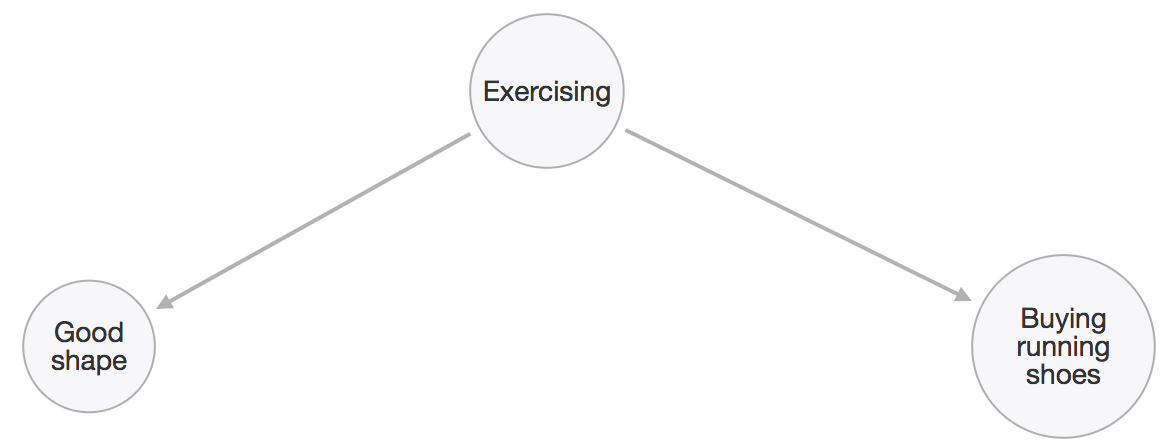
\includegraphics[scale=0.6]{/Users/MauricioGS1/INAOE/Comentarios/Figures/Causal_example.png}
\end{center}
\item Reinforcement Learning (\cite{sutton1998reinforcement}, \cite{gershman2015reinforcement}): An agent learns through exploration and interaction with environment.
\begin{center}
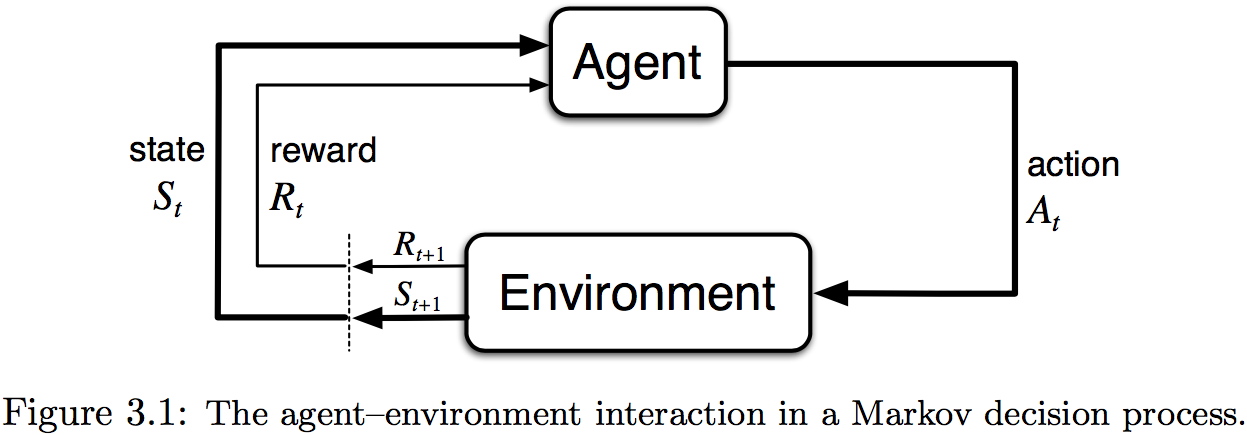
\includegraphics[scale=0.7]{/Users/MauricioGS1/INAOE/Comentarios/Figures/RL.png}\footnote{Image taken from \cite{sutton1998reinforcement}}
\end{center}
\end{itemize}
\subsection*{Where are we standing?}
\begin{itemize}
\item Causal decision theory (\cite{joyce1999foundations}): Making decisions using causal knowledge; i.e. I know that $A$ \textit{causes} $B$, so it can be predicted what will happen if $A$ is chosen, or not, over other options. 
\begin{center}
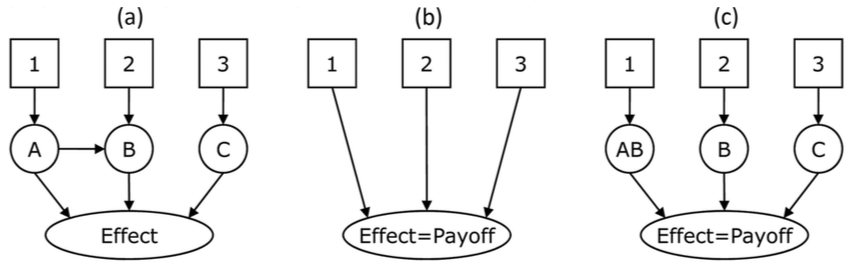
\includegraphics[scale=0.8]{/Users/MauricioGS1/INAOE/Comentarios/Figures/Causal_Decision.png}\footnote{Image taken from \cite{hagmayer2013repeated}}
\end{center}
\item Causal learning through sequential decision making (\cite{hagmayer2013repeated}): Causal learning in humans has been studied in the context of sequental decision-making
\begin{center}
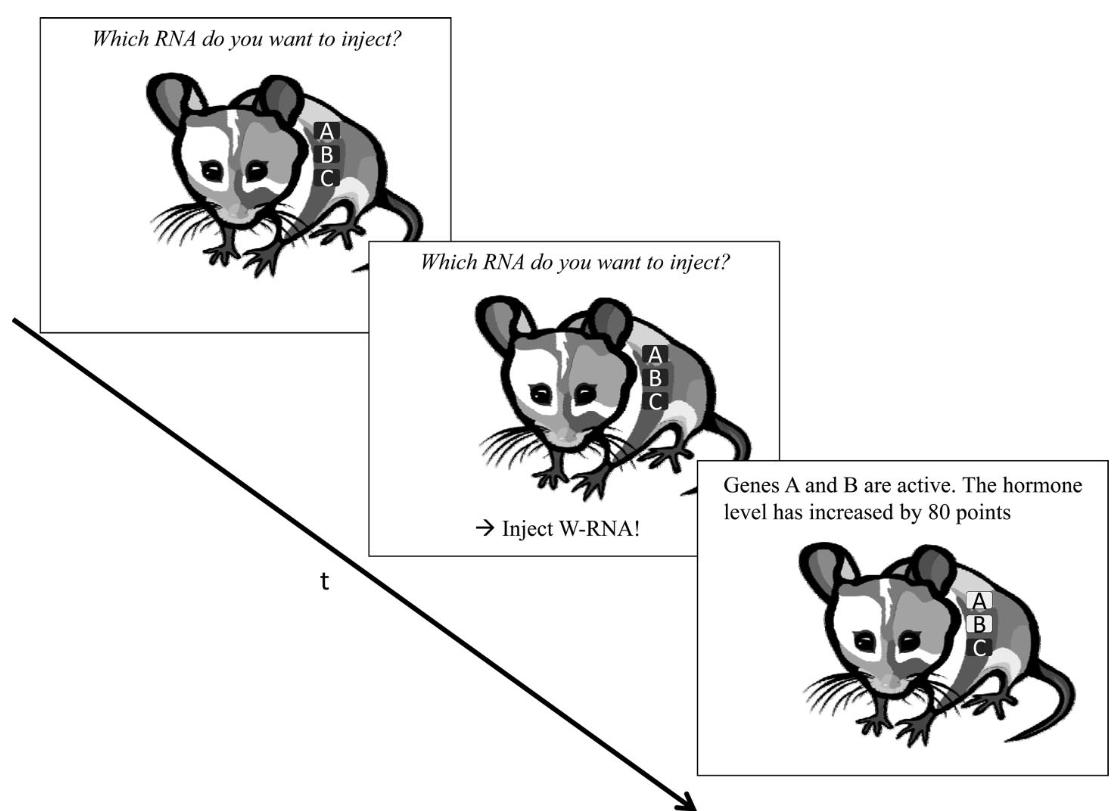
\includegraphics[scale=0.7]{/Users/MauricioGS1/INAOE/Comentarios/Figures/Hagmayer_rats.png}\footnote{Image taken from \cite{hagmayer2013repeated}}
\end{center}
\item On-line learning in causal models(\cite{wellen2012learning}), \cite{garnelo2016towards}):  Causal learning in an on-line setting has been framed in terms of causal graphical models, where in a causal graphical model edges are added or removed in a prediction-error loop
\begin{center}
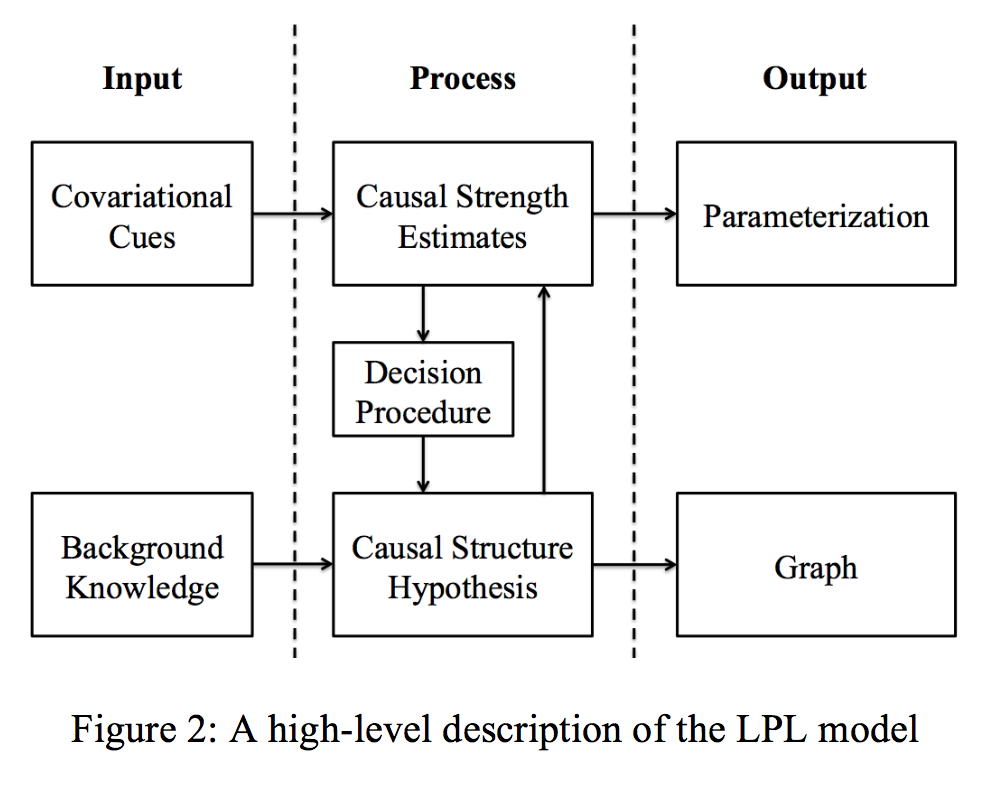
\includegraphics[scale=0.8]{/Users/MauricioGS1/INAOE/Comentarios/Figures/LPL_model.png}\footnote{Image taken from \cite{wellen2012learning}}
\end{center}
\item Decision problems and causal models: \cite{dawid2002influence} show how causal Bayesian Nets can be augmented with decision nodes as to model decision problems that use causal information.
\begin{center}
\includegraphics[scale=0.8]{/Users/MauricioGS1/INAOE/Comentarios/Figures/Influence_diagram.png}\footnote{Image taken from \cite{dawid2002influence}}
\end{center}
\end{itemize}
%And we can think about these areas relating in the following way:
%\begin{center}
%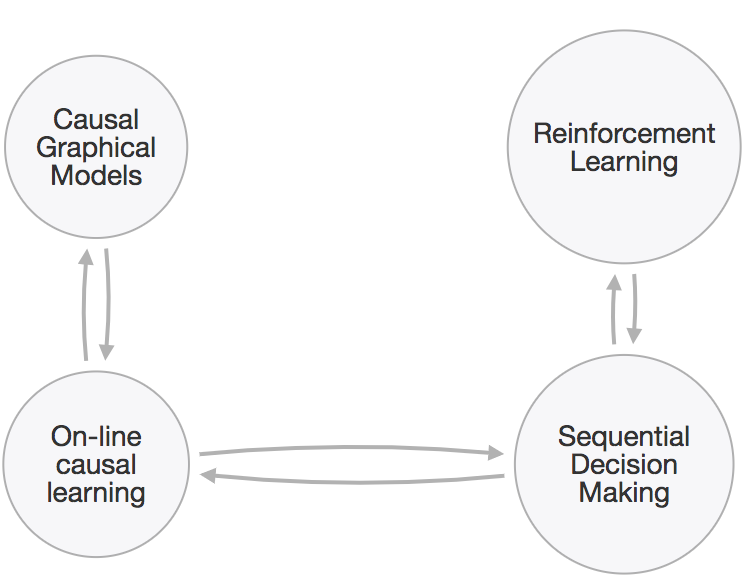
\includegraphics[scale=0.7]{/Users/MauricioGS1/INAOE/Comentarios/Figures/diagrama_eng.png}
%\end{center}

%----------------------------------------------------------------------------------------
%	MOTIVACIÓN
%----------------------------------------------------------------------------------------

\section*{Motivation}
It has been shown by \cite{garnelo2016towards} that causal structure can be learnt from the interaction of an agent with his environment while it learns to perform some task. \\
\begin{center}
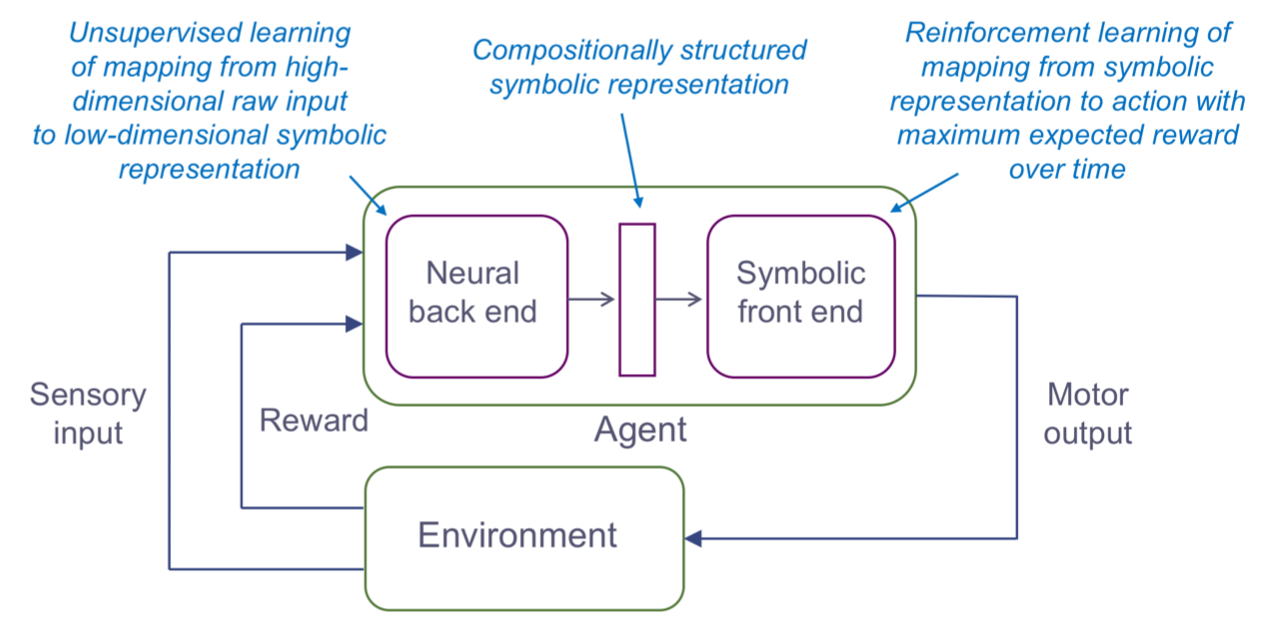
\includegraphics[scale=0.8]{/Users/MauricioGS1/INAOE/Comentarios/Figures/Garnelo.png}\footnote{Image taken from \cite{garnelo2016towards}}
\end{center}
Instead of a fully expresive casual graphical model, they use first-order logic which is somehow restrictive while showing the importance of having some semantics capable of managing causal structure.\\
\begin{center}
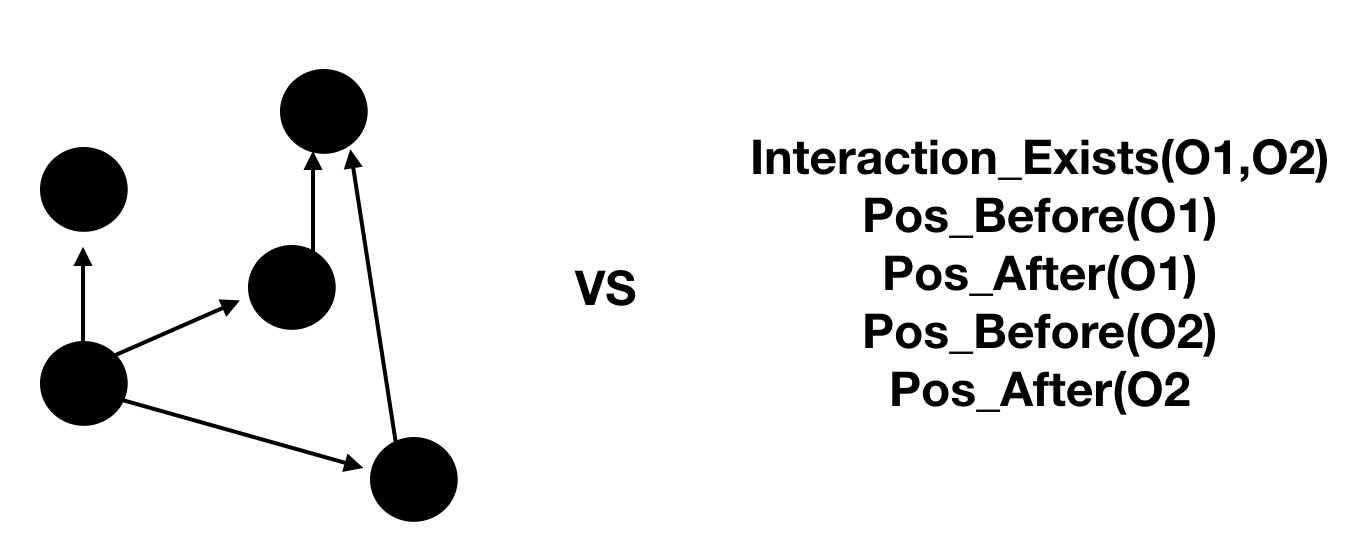
\includegraphics[scale=0.6]{/Users/MauricioGS1/INAOE/Comentarios/Figures/Graph_vs_logic.png}
\end{center}
Meanwhile \cite{wellen2012learning} show how a causal graphical model can be learned on-line by a decision maker through local prediction-error learning.\\ 
\begin{center}
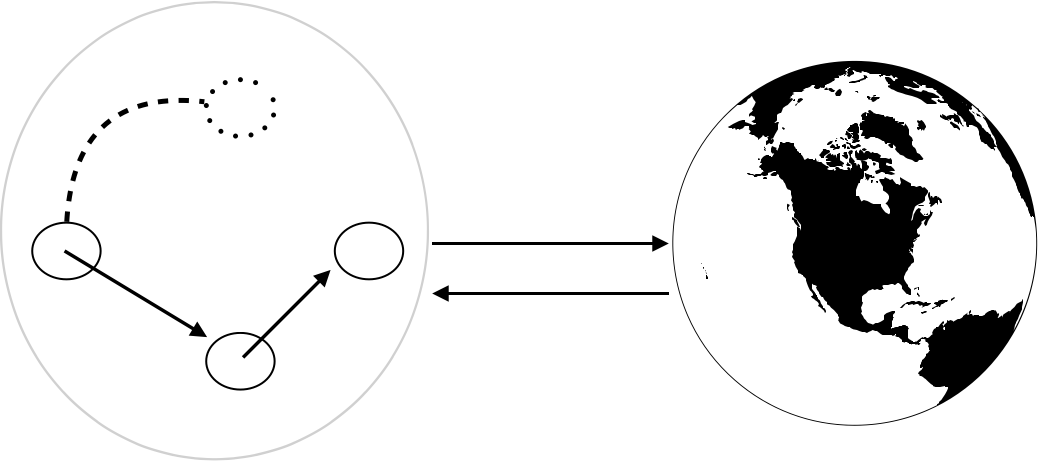
\includegraphics[scale=0.6]{/Users/MauricioGS1/INAOE/Comentarios/Figures/LPL_example_2.png}
\end{center}
From the human psychology side \cite{hagmayer2013repeated} show that our intuitions aren't flawed, because human beings acquire and use causal knowledge while engaging in simple decision-making.
\begin{center}
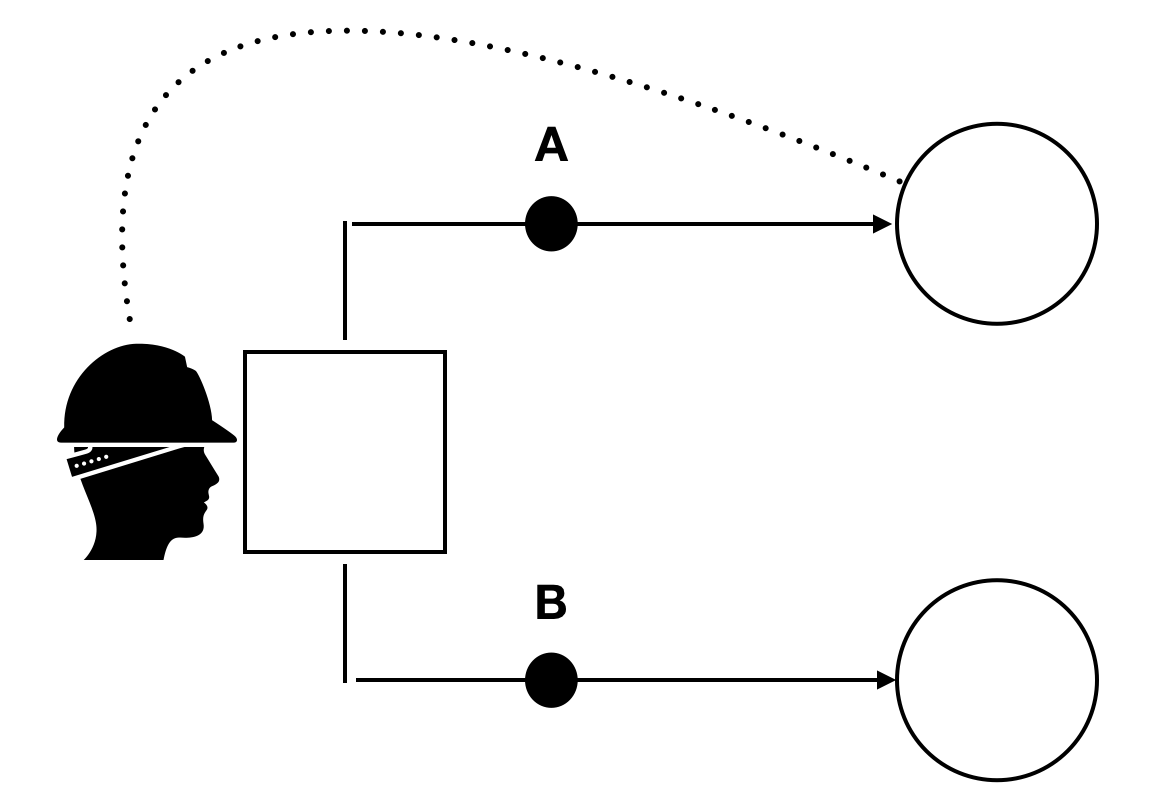
\includegraphics[scale=0.6]{/Users/MauricioGS1/INAOE/Comentarios/Figures/Causal_Feedback.png}
\end{center}
%\\
%\cite{hagmayer2013repeated} asked what would happen with an agent that must learn some particular task instead of only attempting to directly learn causal structure. \\
Each decision made by the agent can be interpreted as an intervention in his environment (\cite{hagmayer2009decision}) which provides information about the world's causal structure.\\
\begin{center}
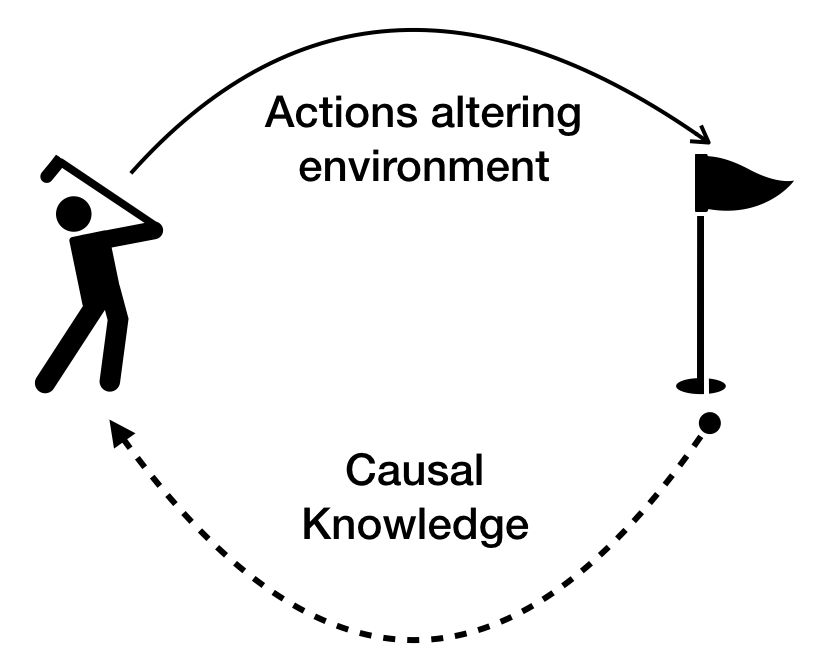
\includegraphics[scale=0.6]{/Users/MauricioGS1/INAOE/Comentarios/Figures/Golf.png}
\end{center}
Learning causal structure will allow the agent to make better decisions because it will be able to consider \textbf{consequences} of his actions, and \textbf{not only reacting} to rewards.\\
\begin{center}
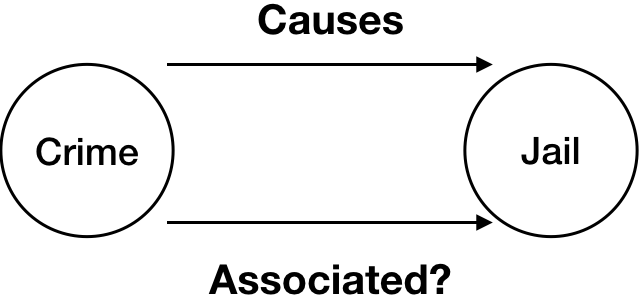
\includegraphics[scale=0.6]{/Users/MauricioGS1/INAOE/Comentarios/Figures/jail.png}
\end{center}
Therefore, we ask ourselves how an agent would learn a causal model in terms of his actions and their consequences? How would this knowledge could be used to make better decisions in the future?
\color{SaddleBrown} % SaddleBrown color for the conclusions to make them stand out
%----------------------------------------------------------------------------------------
%	PROPUESTA
%----------------------------------------------------------------------------------------
\section*{Proposal}
\subsection*{Research question}
Can \textbf{Reinforcement Learning} methods capture a \textbf{causal model} of the environment rather than just an action-outcome mapping as to make \textbf{better decisions}?
\subsection*{Objectives}
\begin{itemize}
\item Defining how to \textbf{learn} causal relations in an \textbf{on-line} setting in terms of actions taken by an agent and their outcomes.
\item Defining how to \textbf{incorporate} the current causal knowledge in order to choose \textbf{better actions}.
\item Defining a way to \textbf{evaluate} how the causal knowledge was used in the decision-making process. We do not want to lose the \textbf{interpretability} of causal graphs.
\item Defining how to \textbf{extract} the acquired causal knowledge to use it in other domains.
\end{itemize}
\subsection*{Proposed Methodology}
My proposal is about incorporating a \textbf{causal model} inside a sequential decision making problem in which an agent has to maximize some reward by \textbf{selecting actions}.\\
\begin{center}
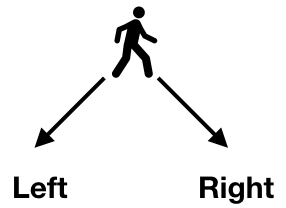
\includegraphics[scale=0.9]{/Users/MauricioGS1/INAOE/Comentarios/Figures/choose_actions.png}
\end{center}
The agent will \textbf{interact} with its environment and receive a \textbf{feedback} signal based on the actions taken by him, which will modify his current causal knowledge.\\
\begin{center}
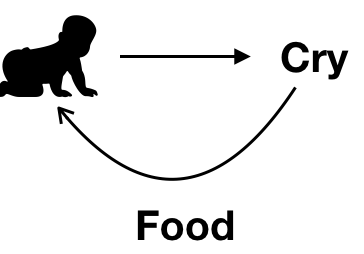
\includegraphics[scale=0.8]{/Users/MauricioGS1/INAOE/Comentarios/Figures/cry.png}
\end{center}
%Using this information, as well as the \textbf{new state} of the world, the internal \textbf{causal model} of the agent will be modified (if needed), either adding or deleting edges or modifying the \textit{causal strength} associated.\\
%\\
Before the next step is taken, the current \textbf{causal knowledge} will be taken into account when \textbf{choosing the next action} together with the current value of each posible action.\\ 
\begin{center}
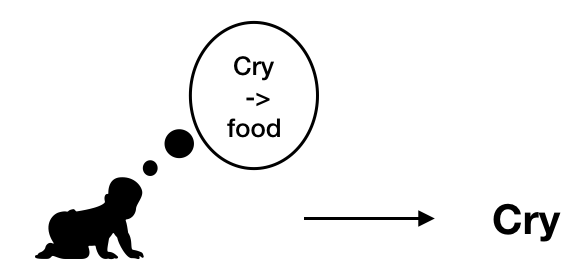
\includegraphics[scale=0.8]{/Users/MauricioGS1/INAOE/Comentarios/Figures/baby.png}
\end{center}
This new action and its outcome will again modify the causal knowledge, which will improve the next action and so on.
\begin{center}
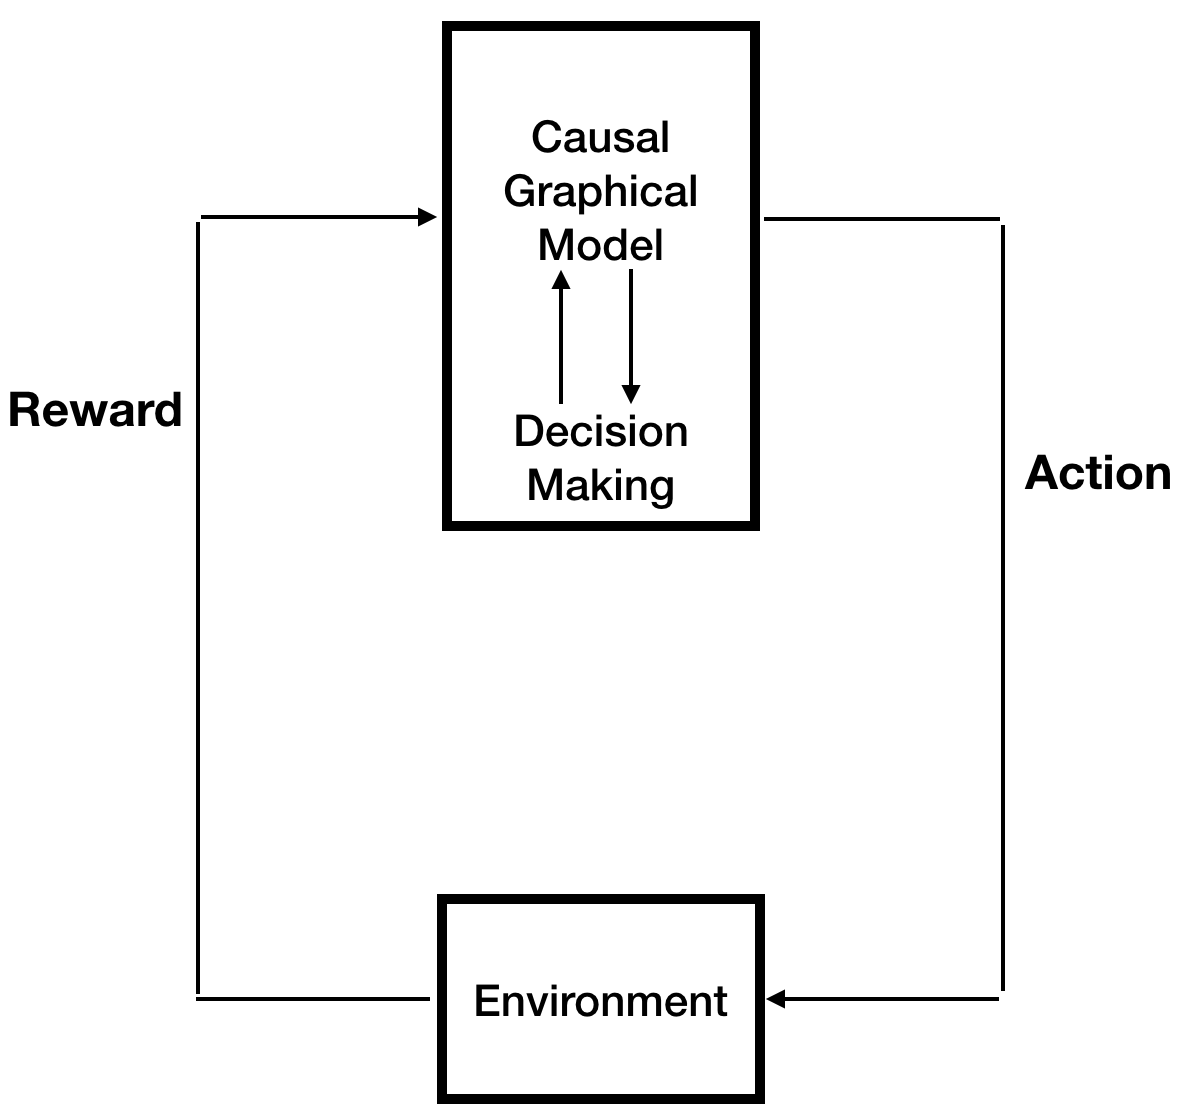
\includegraphics[scale=0.7]{/Users/MauricioGS1/INAOE/Comentarios/Figures/Proposed.png}
\end{center}
\subsection*{Evaluation}
How is this better? Why should we care about learning anything extra if the task is achieved?\\
\\
Causal structures learnt by the agent can be evaluated if compared with an external \textit{real} causal model, or comparing with the initial \textit{prior} causal graph as made by  \cite{hagmayer2013repeated}.
\subsection*{Expected contributions}
\begin{itemize}
\item A framework in which an agent set to learn some task by action-reward can learn causal structure about its environment.
\item An algorithm that learns causal structure in an on-line way.
\item A decision-making procedure that uses current causal knowledge together with action-value estimates.
\end{itemize}
\subsection*{Expected time-line}
\begin{center}
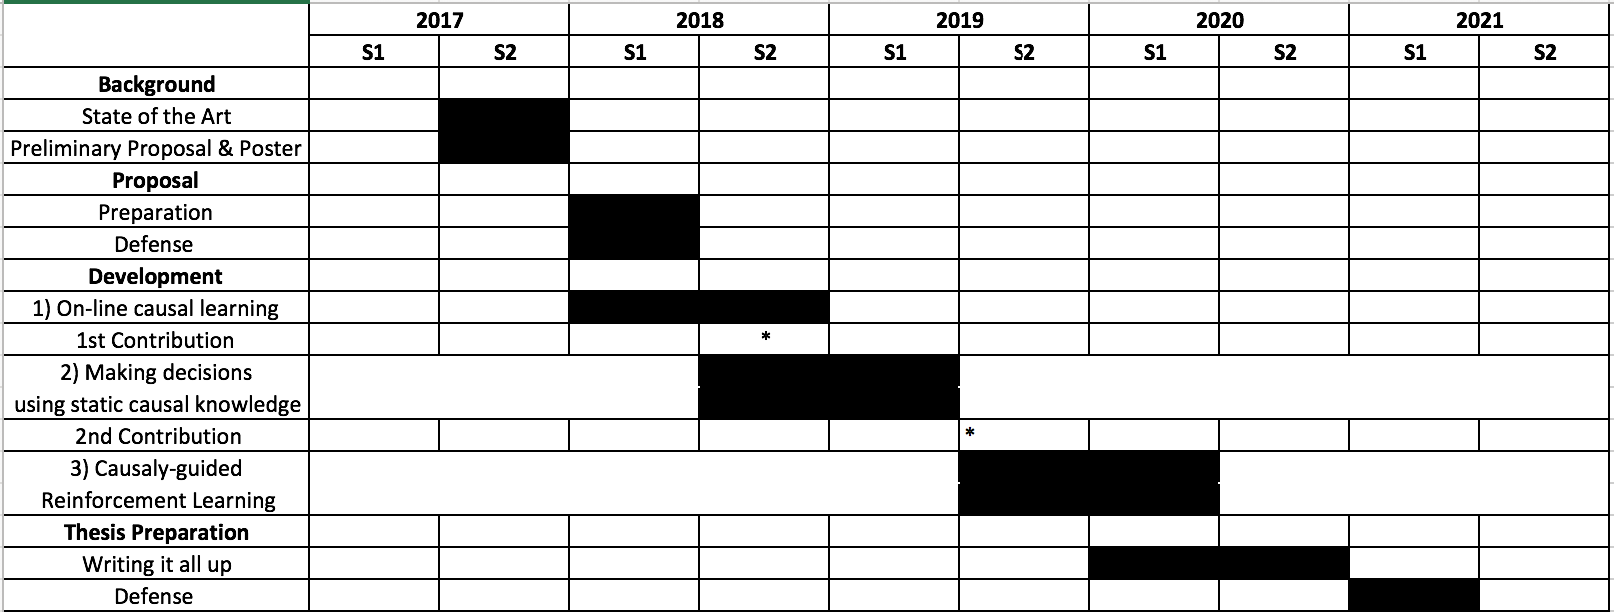
\includegraphics[scale=0.8]{/Users/MauricioGS1/INAOE/Comentarios/Figures/Gantt.png}
\end{center}
%------------------------------------------------------------------------------------------
% BIBLIOGRAPHY
%------------------------------------------------------------------------------------------
\bibliographystyle{apalike}
\bibliography{/Users/MauricioGS1/INAOE/Comentarios/Bibliografia.bib}
\end{multicols}
 %----------------------------------------------------------------------------------------
%	REFERENCES
%----------------------------------------------------------------------------------------
%\begin{minipage}[b]{0.55\linewidth}
%\nocite{*} % Print all references regardless of whether they were cited in the poster or not
%\bibliographystyle{apalike}
%\bibliography{/Users/MauricioGS1/INAOE/Comentarios/Bibliografia.bib}
%\end{minipage}
%\begin{minipage}[b]{0.50\linewidth}
%\subsection*{Expected contribution}
%\begin{itemize}
%\item Build a framework in which an agent set to learn some task by action-reward can learn causal structure about its environment.
%\item Algorithm that learn causal structure in an on-line way.
%\item Using causal knowledge in each step to have better insights in the next decision.
%\end{itemize}
%\subsection*{Expected time-line}
%\begin{itemize}
%\item May 2018: Formal proposal.
%\item August 2018: Proposal defense.
%\%item December 2018: On-line causal learning module
%\end{itemize}
%\end{minipage}
\end{document}
